% Copyright (C) 2021 Erwin Müller <erwin@muellerpublic.de>
% Released as open-source under the Apache License, Version 2.0.
%
% ****************************************************************************
% ANL-OpenCL :: Docs
% ****************************************************************************
%
% Copyright (C) 2021 Erwin Müller <erwin@muellerpublic.de>
%
% Licensed under the Apache License, Version 2.0 (the "License");
% you may not use this file except in compliance with the License.
% You may obtain a copy of the License at
%
%      http://www.apache.org/licenses/LICENSE-2.0
%
% Unless required by applicable law or agreed to in writing, software
% distributed under the License is distributed on an "AS IS" BASIS,
% WITHOUT WARRANTIES OR CONDITIONS OF ANY KIND, either express or implied.
% See the License for the specific language governing permissions and
% limitations under the License.
%
% ****************************************************************************
% ANL-OpenCL :: Docs is a derivative work based on Josua Tippetts' C++ library:
% http://accidentalnoise.sourceforge.net/index.html
% ****************************************************************************
%
% Copyright (C) 2011 Joshua Tippetts
%
%   This software is provided 'as-is', without any express or implied
%   warranty.  In no event will the authors be held liable for any damages
%   arising from the use of this software.
%
%   Permission is granted to anyone to use this software for any purpose,
%   including commercial applications, and to alter it and redistribute it
%   freely, subject to the following restrictions:
%
%   1. The origin of this software must not be misrepresented; you must not
%      claim that you wrote the original software. If you use this software
%      in a product, an acknowledgment in the product documentation would be
%      appreciated but is not required.
%   2. Altered source versions must be plainly marked as such, and must not be
%      misrepresented as being the original software.
%   3. This notice may not be removed or altered from any source distribution.
%
%
% ****************************************************************************
% ANL-OpenCL :: Docs bundles and uses the RandomCL library:
% https://github.com/bstatcomp/RandomCL
% ****************************************************************************
%
% BSD 3-Clause License
%
% Copyright (c) 2018, Tadej Ciglarič, Erik Štrumbelj, Rok Češnovar. All rights reserved.
%
% Redistribution and use in source and binary forms, with or without modification, are permitted provided that the following conditions are met:
%
% * Redistributions of source code must retain the above copyright notice, this list of conditions and the following disclaimer.
%
% * Redistributions in binary form must reproduce the above copyright notice, this list of conditions and the following disclaimer in the documentation and/or other materials provided with the distribution.
%
% * Neither the name of the copyright holder nor the names of its contributors may be used to endorse or promote products derived from this software without specific prior written permission.
%
% THIS SOFTWARE IS PROVIDED BY THE COPYRIGHT HOLDERS AND CONTRIBUTORS "AS IS" AND ANY EXPRESS OR IMPLIED WARRANTIES, INCLUDING, BUT NOT LIMITED TO, THE IMPLIED WARRANTIES OF MERCHANTABILITY AND FITNESS FOR A PARTICULAR PURPOSE ARE DISCLAIMED. IN NO EVENT SHALL THE COPYRIGHT HOLDER OR CONTRIBUTORS BE LIABLE FOR ANY DIRECT, INDIRECT, INCIDENTAL, SPECIAL, EXEMPLARY, OR CONSEQUENTIAL DAMAGES (INCLUDING, BUT NOT LIMITED TO, PROCUREMENT OF SUBSTITUTE GOODS OR SERVICES; LOSS OF USE, DATA, OR PROFITS; OR BUSINESS INTERRUPTION) HOWEVER CAUSED AND ON ANY THEORY OF LIABILITY, WHETHER IN CONTRACT, STRICT LIABILITY, OR TORT (INCLUDING NEGLIGENCE OR OTHERWISE) ARISING IN ANY WAY OUT OF THE USE OF THIS SOFTWARE, EVEN IF ADVISED OF THE POSSIBILITY OF SUCH DAMAGE.

\documentclass[10pt,abstract=yes,toc=flat]{docusimple}
% Copyright (C) 2021 Erwin Müller <erwin@muellerpublic.de>
% Released as open-source under the Apache License, Version 2.0.
%
% ****************************************************************************
% ANL-OpenCL :: Bundle POM
% ****************************************************************************
%
% Copyright (C) 2021 Erwin Müller <erwin@muellerpublic.de>
%
% Licensed under the Apache License, Version 2.0 (the "License");
% you may not use this file except in compliance with the License.
% You may obtain a copy of the License at
%
%      http://www.apache.org/licenses/LICENSE-2.0
%
% Unless required by applicable law or agreed to in writing, software
% distributed under the License is distributed on an "AS IS" BASIS,
% WITHOUT WARRANTIES OR CONDITIONS OF ANY KIND, either express or implied.
% See the License for the specific language governing permissions and
% limitations under the License.
%
% ****************************************************************************
% ANL-OpenCL :: Bundle POM is a derivative work based on Josua Tippetts' C++ library:
% http://accidentalnoise.sourceforge.net/index.html
% ****************************************************************************
%
% Copyright (C) 2011 Joshua Tippetts
%
%   This software is provided 'as-is', without any express or implied
%   warranty.  In no event will the authors be held liable for any damages
%   arising from the use of this software.
%
%   Permission is granted to anyone to use this software for any purpose,
%   including commercial applications, and to alter it and redistribute it
%   freely, subject to the following restrictions:
%
%   1. The origin of this software must not be misrepresented; you must not
%      claim that you wrote the original software. If you use this software
%      in a product, an acknowledgment in the product documentation would be
%      appreciated but is not required.
%   2. Altered source versions must be plainly marked as such, and must not be
%      misrepresented as being the original software.
%   3. This notice may not be removed or altered from any source distribution.
%
%
% ****************************************************************************
% ANL-OpenCL :: Bundle POM bundles and uses the RandomCL library:
% https://github.com/bstatcomp/RandomCL
% ****************************************************************************
%
% BSD 3-Clause License
%
% Copyright (c) 2018, Tadej Ciglarič, Erik Štrumbelj, Rok Češnovar. All rights reserved.
%
% Redistribution and use in source and binary forms, with or without modification, are permitted provided that the following conditions are met:
%
% * Redistributions of source code must retain the above copyright notice, this list of conditions and the following disclaimer.
%
% * Redistributions in binary form must reproduce the above copyright notice, this list of conditions and the following disclaimer in the documentation and/or other materials provided with the distribution.
%
% * Neither the name of the copyright holder nor the names of its contributors may be used to endorse or promote products derived from this software without specific prior written permission.
%
% THIS SOFTWARE IS PROVIDED BY THE COPYRIGHT HOLDERS AND CONTRIBUTORS "AS IS" AND ANY EXPRESS OR IMPLIED WARRANTIES, INCLUDING, BUT NOT LIMITED TO, THE IMPLIED WARRANTIES OF MERCHANTABILITY AND FITNESS FOR A PARTICULAR PURPOSE ARE DISCLAIMED. IN NO EVENT SHALL THE COPYRIGHT HOLDER OR CONTRIBUTORS BE LIABLE FOR ANY DIRECT, INDIRECT, INCIDENTAL, SPECIAL, EXEMPLARY, OR CONSEQUENTIAL DAMAGES (INCLUDING, BUT NOT LIMITED TO, PROCUREMENT OF SUBSTITUTE GOODS OR SERVICES; LOSS OF USE, DATA, OR PROFITS; OR BUSINESS INTERRUPTION) HOWEVER CAUSED AND ON ANY THEORY OF LIABILITY, WHETHER IN CONTRACT, STRICT LIABILITY, OR TORT (INCLUDING NEGLIGENCE OR OTHERWISE) ARISING IN ANY WAY OUT OF THE USE OF THIS SOFTWARE, EVEN IF ADVISED OF THE POSSIBILITY OF SUCH DAMAGE.

\usepackage{listings} 
\usepackage{xcolor}
\usepackage{imakeidx}
\usepackage{subcaption}
\makeindex

\definecolor{codegreen}{rgb}{0,0.6,0}
\definecolor{codegray}{rgb}{0.5,0.5,0.5}
\definecolor{codepurple}{rgb}{0.58,0,0.82}
\definecolor{backcolour}{rgb}{0.95,0.95,0.92}
\definecolor{myGreen}{rgb}{0.1,0.6,0.2}

\lstdefinelanguage[]{OpenCL}[ANSI]{C}{
    sensitive=false,
    morekeywords={kernel,global,write_only,read_only},
    alsoletter={\$},
    morekeywords=[2]{\$insert_localMapRange,\$localSize,\$z},
    morecomment=[l][{\color{myGreen}}]{\#}
}

\lstdefinestyle{c-my}{
    backgroundcolor=\color{backcolour},   
    commentstyle=\color{codegreen},
    keywordstyle=\color{magenta},
    keywordstyle={[2]\color{myGreen}},
    numberstyle=\tiny\color{codegray},
    stringstyle=\color{codepurple},
    basicstyle=\ttfamily\footnotesize,
    breakatwhitespace=false,         
    breaklines=true,                 
    captionpos=b,                    
    keepspaces=true,                 
    numbers=left,                    
    numbersep=0pt,                  
    showspaces=false,                
    showstringspaces=false,
    showtabs=false,                  
    tabsize=2
}

\lstset{style=c-my}


\begin{document}
% title page
% 
\titlehead{%
}
%
\subject{\SubjectStyle{%
ANL-OpenCL}}
%
\title{%
Documentation}
%
\subtitle{%
}
%
\author{\AuthorStyle{%
Erwin Müller}}
%
\date{\DateStyle{%
\today}}
%
\publishers{\PublishersStyle{%
\url{https://anl-opencl.anrisoftware.com/}}}
%
\renewcommand{\TheHeadingLogo}{%

\includegraphics[height=1em]{logo.png}}
%
\renewcommand{\TheHeadingAuthor}{%
}
%
%\thanks{footnote }
%
%\lowertitleback{}
%
\uppertitleback{%
}
%
\dedication{\DedicationStyle{%
}}
%
\newcommand{\TheAbstract}{
\begin{center}
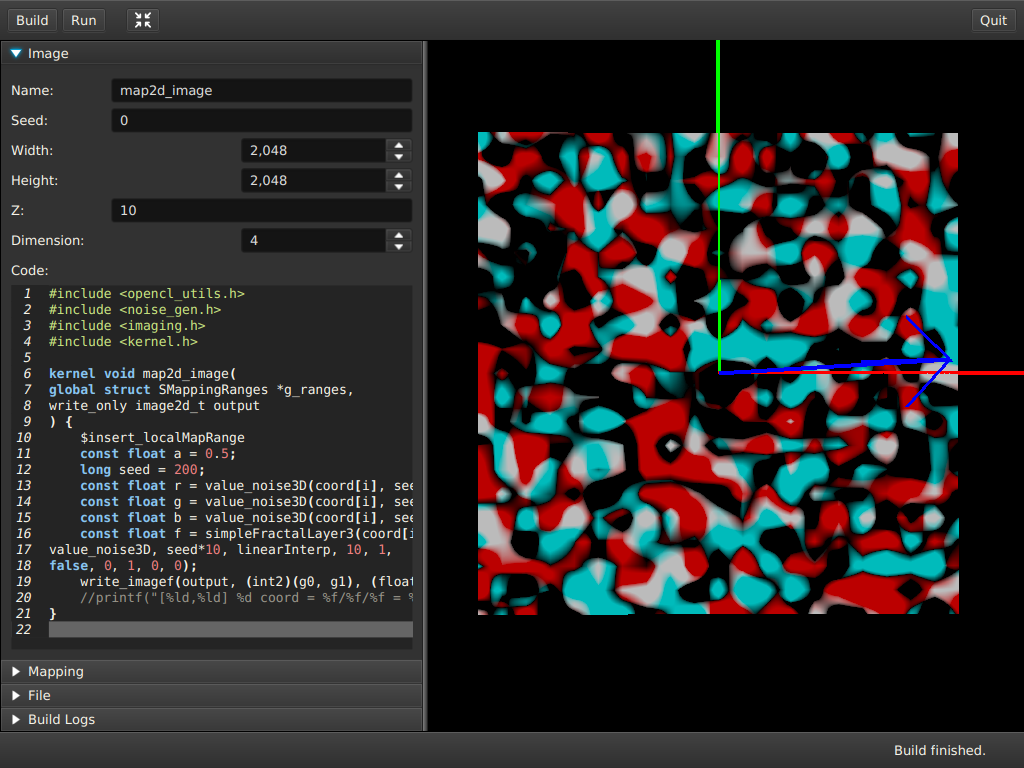
\includegraphics[width=0.8\textwidth]{Screenshot_20211121_152848.png}
\end{center}
The purpose of this document is to describe the \ANLOpenCL/ library, how to
use it to create noise images and how to use the bundled app.
} 
%

\maketitle
\TheAbstract{}
\tableofcontents

% Copyright (C) 2021 Erwin Müller <erwin@muellerpublic.de>
% Released as open-source under the Apache License, Version 2.0.
%
% ****************************************************************************
% ANL-OpenCL :: Docs
% ****************************************************************************
%
% Copyright (C) 2021 Erwin Müller <erwin@muellerpublic.de>
%
% Licensed under the Apache License, Version 2.0 (the "License");
% you may not use this file except in compliance with the License.
% You may obtain a copy of the License at
%
%      http://www.apache.org/licenses/LICENSE-2.0
%
% Unless required by applicable law or agreed to in writing, software
% distributed under the License is distributed on an "AS IS" BASIS,
% WITHOUT WARRANTIES OR CONDITIONS OF ANY KIND, either express or implied.
% See the License for the specific language governing permissions and
% limitations under the License.
%
% ****************************************************************************
% ANL-OpenCL :: Docs is a derivative work based on Josua Tippetts' C++ library:
% http://accidentalnoise.sourceforge.net/index.html
% ****************************************************************************
%
% Copyright (C) 2011 Joshua Tippetts
%
%   This software is provided 'as-is', without any express or implied
%   warranty.  In no event will the authors be held liable for any damages
%   arising from the use of this software.
%
%   Permission is granted to anyone to use this software for any purpose,
%   including commercial applications, and to alter it and redistribute it
%   freely, subject to the following restrictions:
%
%   1. The origin of this software must not be misrepresented; you must not
%      claim that you wrote the original software. If you use this software
%      in a product, an acknowledgment in the product documentation would be
%      appreciated but is not required.
%   2. Altered source versions must be plainly marked as such, and must not be
%      misrepresented as being the original software.
%   3. This notice may not be removed or altered from any source distribution.
%
%
% ****************************************************************************
% ANL-OpenCL :: Docs bundles and uses the RandomCL library:
% https://github.com/bstatcomp/RandomCL
% ****************************************************************************
%
% BSD 3-Clause License
%
% Copyright (c) 2018, Tadej Ciglarič, Erik Štrumbelj, Rok Češnovar. All rights reserved.
%
% Redistribution and use in source and binary forms, with or without modification, are permitted provided that the following conditions are met:
%
% * Redistributions of source code must retain the above copyright notice, this list of conditions and the following disclaimer.
%
% * Redistributions in binary form must reproduce the above copyright notice, this list of conditions and the following disclaimer in the documentation and/or other materials provided with the distribution.
%
% * Neither the name of the copyright holder nor the names of its contributors may be used to endorse or promote products derived from this software without specific prior written permission.
%
% THIS SOFTWARE IS PROVIDED BY THE COPYRIGHT HOLDERS AND CONTRIBUTORS "AS IS" AND ANY EXPRESS OR IMPLIED WARRANTIES, INCLUDING, BUT NOT LIMITED TO, THE IMPLIED WARRANTIES OF MERCHANTABILITY AND FITNESS FOR A PARTICULAR PURPOSE ARE DISCLAIMED. IN NO EVENT SHALL THE COPYRIGHT HOLDER OR CONTRIBUTORS BE LIABLE FOR ANY DIRECT, INDIRECT, INCIDENTAL, SPECIAL, EXEMPLARY, OR CONSEQUENTIAL DAMAGES (INCLUDING, BUT NOT LIMITED TO, PROCUREMENT OF SUBSTITUTE GOODS OR SERVICES; LOSS OF USE, DATA, OR PROFITS; OR BUSINESS INTERRUPTION) HOWEVER CAUSED AND ON ANY THEORY OF LIABILITY, WHETHER IN CONTRACT, STRICT LIABILITY, OR TORT (INCLUDING NEGLIGENCE OR OTHERWISE) ARISING IN ANY WAY OUT OF THE USE OF THIS SOFTWARE, EVEN IF ADVISED OF THE POSSIBILITY OF SUCH DAMAGE.

\section{App}

\begin{figure}
\centering
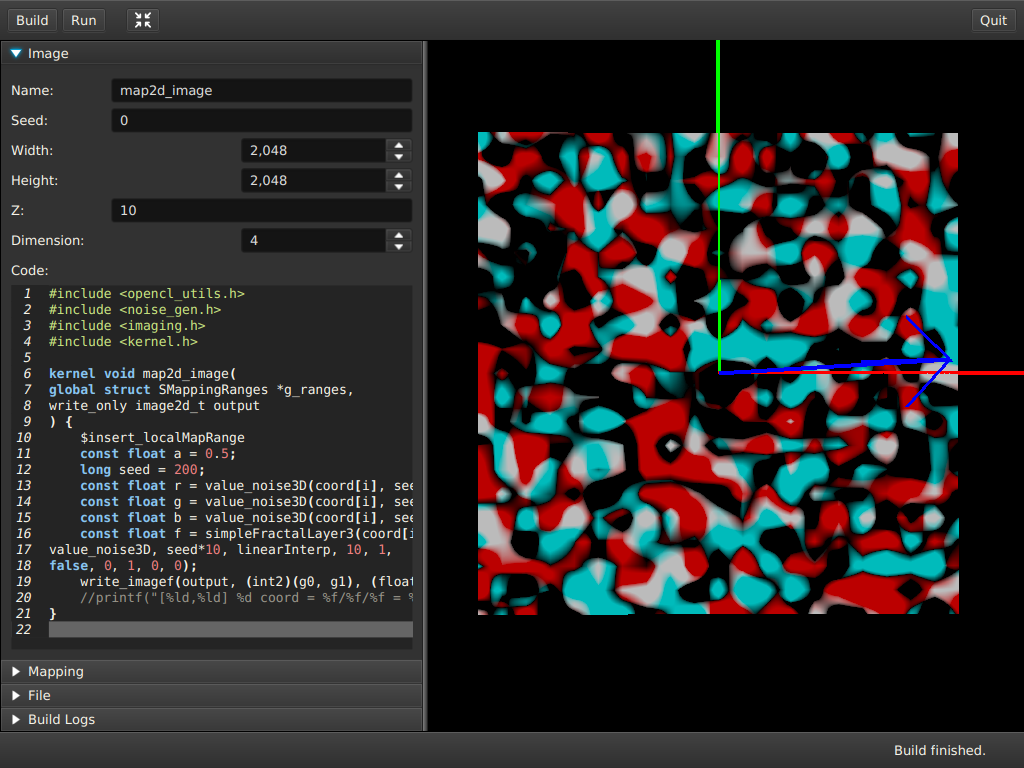
\includegraphics[width=0.4\textwidth]{Screenshot_20211121_152848.png}
\caption{Screenshot of the app version 0.0.2}\label{fig:app_screenshot}
\end{figure}

The bundled app is a graphical user interface to enter the kernel code, build
it and generate a preview of the noise image. It is implemented 
in Java and JMonkeyEngine 3. The goal of the app is to quickly prototype
noise images with kernel code. The goal is not to provide an IDE or an advanced
code editor. The app is divided into two parts. One part is to enter the kernel code and
parameters and other other part is to display the generated images.

\subsection{Toolbar}

\begin{figure}[h]
\centering

\includegraphics[width=0.4\textwidth]{imgs/toolbar-screenshot-0.png}
\caption{Toolbar}\label{fig:toolbar-screenshot-0}
\end{figure}

The toolbar have buttons for the most common functions.

\subsubsection{Build}

\begin{figure}[h]
\centering

\includegraphics{imgs/toolbar-build-0.png}
\caption{Toolbar Build Button}\label{fig:toolbar-build-0}
\end{figure}

The Build button will build the kernel code and display the generated image
according to the parameters.

\subsubsection{Reset Camera}

\begin{figure}[h]
\centering

\includegraphics{imgs/toolbar-reset-camera-0.png}
\caption{Toolbar Build Button}\label{fig:toolbar-reset-camera-0}
\end{figure}

The Reset Camera button will reset the camera to the default position and zoom.
Key shortcut F10.

\subsubsection{Quit}

\begin{figure}[h]
\centering

\includegraphics{imgs/toolbar-quit-0.png}
\caption{Toolbar Build Button}\label{fig:toolbar-quit-0}
\end{figure}

The Quit button will exit the app. Key shortcut Ctrl-Q.

\label{sec:image}\subsection{Image}

\begin{figure}[h]
\centering
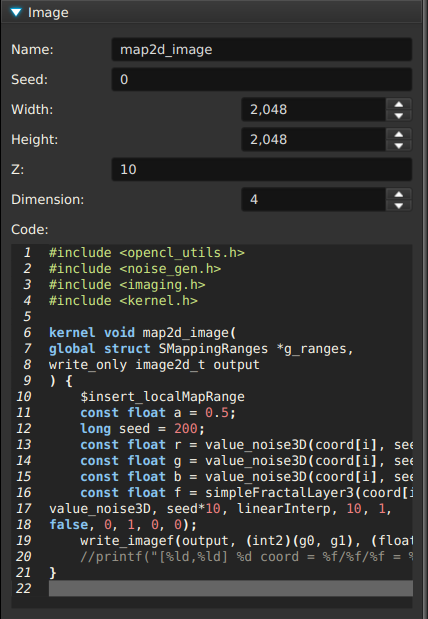
\includegraphics[width=0.4\textwidth]{imgs/main-image-0.png}
\caption{Image}\label{fig:main-image-0}
\end{figure}

The image window have the image parameters and the kernel code.

\subsubsection{Name}

The name of the kernel to build.

\subsubsection{Seed}

The seed number.

\subsubsection{Width}

The width of the image in pixels.

\subsubsection{Height}

The height of the image in pixels.

\subsubsection{Z}

The Z value.

\subsubsection{Dimension}

The count of float numbers of each coordinate. Different noise functions
expect to have the correct dimension of the coordinates available.

\begin{description}
\item[2D] requires dimension of 2 for \texttt{float2};
\item[3D] requires dimension of 4 for \texttt{float3};
\item[4D] requires dimension of 4 for \texttt{float4};
\item[6D] requires dimension of 8 for \texttt{float8};
\end{description}

\label{sec:mapping}\subsection{Mapping}

\begin{figure}[h]
\centering
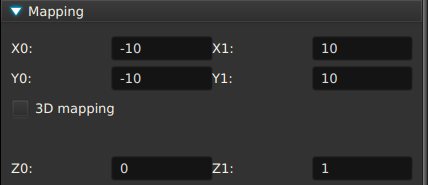
\includegraphics[width=0.4\textwidth]{imgs/main-mapping-0.png}
\caption{Image}\label{fig:main-mapping-0}
\end{figure}

The mapping window have the parameters to map coordinates.

\subsubsection{3D mapping}

If enabled then the mapping is done in 3D and the function \texttt{map3D} must be used.

\subsection{Scene Window}

\begin{figure}[h]
\centering
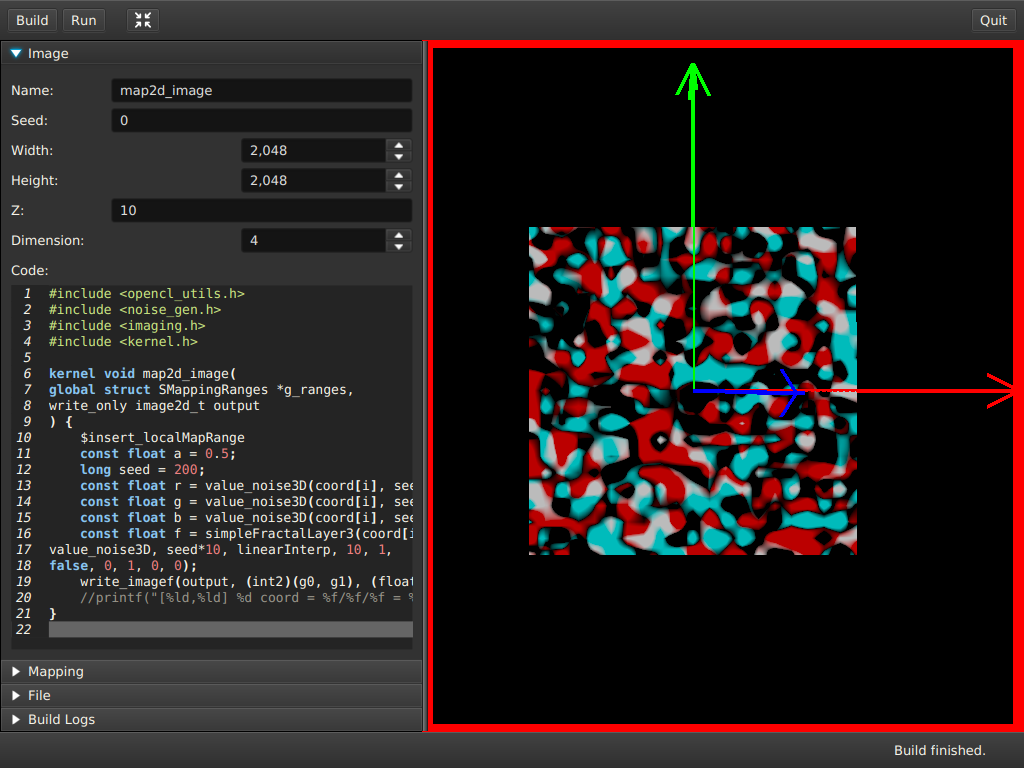
\includegraphics[width=0.4\textwidth]{imgs/main-scene-0.png}
\caption{Image}\label{fig:main-scene-0}
\end{figure}

The scene window shows the generated images. The scene can be moved and zoomed
with the mouse.

\begin{description}
\item[Middle Mouse] moving the scene;
\item[Mouse Wheel] zooming the scene;
\end{description}


\section{API}

This section documents the C functions and types that can be used in \ANLOpenCL/.

% Copyright (C) 2021 Erwin Müller <erwin@muellerpublic.de>
% Released as open-source under the Apache License, Version 2.0.
%
% ****************************************************************************
% ANL-OpenCL :: Docs
% ****************************************************************************
%
% Copyright (C) 2021 Erwin Müller <erwin@muellerpublic.de>
%
% Licensed under the Apache License, Version 2.0 (the "License");
% you may not use this file except in compliance with the License.
% You may obtain a copy of the License at
%
%      http://www.apache.org/licenses/LICENSE-2.0
%
% Unless required by applicable law or agreed to in writing, software
% distributed under the License is distributed on an "AS IS" BASIS,
% WITHOUT WARRANTIES OR CONDITIONS OF ANY KIND, either express or implied.
% See the License for the specific language governing permissions and
% limitations under the License.
%
% ****************************************************************************
% ANL-OpenCL :: Docs is a derivative work based on Josua Tippetts' C++ library:
% http://accidentalnoise.sourceforge.net/index.html
% ****************************************************************************
%
% Copyright (C) 2011 Joshua Tippetts
%
%   This software is provided 'as-is', without any express or implied
%   warranty.  In no event will the authors be held liable for any damages
%   arising from the use of this software.
%
%   Permission is granted to anyone to use this software for any purpose,
%   including commercial applications, and to alter it and redistribute it
%   freely, subject to the following restrictions:
%
%   1. The origin of this software must not be misrepresented; you must not
%      claim that you wrote the original software. If you use this software
%      in a product, an acknowledgment in the product documentation would be
%      appreciated but is not required.
%   2. Altered source versions must be plainly marked as such, and must not be
%      misrepresented as being the original software.
%   3. This notice may not be removed or altered from any source distribution.
%
%
% ****************************************************************************
% ANL-OpenCL :: Docs bundles and uses the RandomCL library:
% https://github.com/bstatcomp/RandomCL
% ****************************************************************************
%
% BSD 3-Clause License
%
% Copyright (c) 2018, Tadej Ciglarič, Erik Štrumbelj, Rok Češnovar. All rights reserved.
%
% Redistribution and use in source and binary forms, with or without modification, are permitted provided that the following conditions are met:
%
% * Redistributions of source code must retain the above copyright notice, this list of conditions and the following disclaimer.
%
% * Redistributions in binary form must reproduce the above copyright notice, this list of conditions and the following disclaimer in the documentation and/or other materials provided with the distribution.
%
% * Neither the name of the copyright holder nor the names of its contributors may be used to endorse or promote products derived from this software without specific prior written permission.
%
% THIS SOFTWARE IS PROVIDED BY THE COPYRIGHT HOLDERS AND CONTRIBUTORS "AS IS" AND ANY EXPRESS OR IMPLIED WARRANTIES, INCLUDING, BUT NOT LIMITED TO, THE IMPLIED WARRANTIES OF MERCHANTABILITY AND FITNESS FOR A PARTICULAR PURPOSE ARE DISCLAIMED. IN NO EVENT SHALL THE COPYRIGHT HOLDER OR CONTRIBUTORS BE LIABLE FOR ANY DIRECT, INDIRECT, INCIDENTAL, SPECIAL, EXEMPLARY, OR CONSEQUENTIAL DAMAGES (INCLUDING, BUT NOT LIMITED TO, PROCUREMENT OF SUBSTITUTE GOODS OR SERVICES; LOSS OF USE, DATA, OR PROFITS; OR BUSINESS INTERRUPTION) HOWEVER CAUSED AND ON ANY THEORY OF LIABILITY, WHETHER IN CONTRACT, STRICT LIABILITY, OR TORT (INCLUDING NEGLIGENCE OR OTHERWISE) ARISING IN ANY WAY OUT OF THE USE OF THIS SOFTWARE, EVEN IF ADVISED OF THE POSSIBILITY OF SUCH DAMAGE.

\subsection{OpenCL Kernel}

The basic structure of a kernel is give as an example in listings \ref{lst:kernel_example}.
The kernel expects two parameters to generale an image as a texture. The first
are the \ANLOpenCLTypeIndex{SMappingRanges} that contains the parameters of the mapping
as entered by the user on the Mapping \ref{sec:mapping} window. The second parameter
is the \ANLOpenCLTypeIndex{image2d\_t} image output.

The kernel code can contain variables that are inserted before the code is build.
One of those variables is \ANLOpenCLTypeIndex{\$insert\_localMapRange}. This variable
is replaced with the code in listings \ref{lst:insert_local_map_range}.
\ANLOpenCLType{\$insert\_localMapRange} contains code that divides the coordinates
space given in the mapping ranges into small peaces and allows the noise functions
to operate in the local group on the divided part. After this code was inserted 
the \code{const int i} variable contains the current index in the \code{vector3 coord}
variable, i.e. reading the coordinate from the position \code{coord[i]} will return
the correct coordinate in the local group. Additionally, the variable
\code{struct SMappingRanges ranges} will contain the local mapping ranges.

The variable \ANLOpenCLTypeIndex{\$localSize} contains the size of the part of the
image that we want to process in pixels. Currently it is set to a maximum size of 32.
That means that an image of the size 1024x1024 is divided into 32x32 ($1024/32=32$) parts
with the size of 32x32 pixels. Each noise function will be called in the local group
only on the 32x32 pixels part.

The variable \ANLOpenCLTypeIndex{\$z} contains the Z value from the Image \ref{sec:image} section.

\begin{lstlisting}[caption={Kernel Example},label={lst:kernel_example},language=OpenCL]
#include <opencl_utils.h>
#include <noise_gen.h>
#include <imaging.h>
#include <kernel.h>

kernel void map2d_image(
global struct SMappingRanges *g_ranges,
write_only image2d_t output
) {
    $insert_localMapRange
    const float a = 0.5;
    long seed = 200;
    const float r = value_noise3D(coord[i], seed, linearInterp);
    const float g = value_noise3D(coord[i], seed*2, linearInterp);
    const float b = value_noise3D(coord[i], seed*2, linearInterp);
    const float f = simpleFractalLayer3(coord[i], 
value_noise3D, seed*10, linearInterp, 10, 1, 
false, 0, 1, 0, 0);
    write_imagef(output, (int2)(g0, g1), (float4)(r*f, g*f, b*f, a));
}
\end{lstlisting}

\begin{lstlisting}[caption={Local Map Range Code},label={lst:insert_local_map_range},language=OpenCL]
const size_t g0 = get_global_id(0);
const size_t g1 = get_global_id(1);
const size_t w = get_global_size(0);
const size_t h = get_global_size(1);
const size_t l0 = get_local_id(0);
const size_t l1 = get_local_id(1);
const size_t lw = get_local_size(0);
const size_t lh = get_local_size(1);
local vector3 coord[$localSize * $localSize];
local struct SMappingRanges ranges;
if (l0 == 0 && l1 == 0) {
    const REAL sw = (g_ranges->mapx1 - g_ranges->mapx0) / w;
    const REAL sh = (g_ranges->mapy1 - g_ranges->mapy0) / h;
    const REAL x0 = g_ranges->mapx0 + g0 * sw;
    const REAL x1 = g_ranges->mapx0 + g0 * sw + sw * lw;
    const REAL y0 = g_ranges->mapy0 + g1 * sh;
    const REAL y1 = g_ranges->mapy0 + g1 * sh + sh * lh;
    set_ranges_map2D(&ranges, x0, x1, y0, y1);
    map2D(coord, calc_seamless_none, ranges, lw, lh, $z);
}
work_group_barrier(CLK_LOCAL_MEM_FENCE);
const int i = (l0 + l1 * lh);
\end{lstlisting}

% Copyright (C) 2021 Erwin Müller <erwin@muellerpublic.de>
% Released as open-source under the Apache License, Version 2.0.
%
% ****************************************************************************
% ANL-OpenCL :: Docs
% ****************************************************************************
%
% Copyright (C) 2021 Erwin Müller <erwin@muellerpublic.de>
%
% Licensed under the Apache License, Version 2.0 (the "License");
% you may not use this file except in compliance with the License.
% You may obtain a copy of the License at
%
%      http://www.apache.org/licenses/LICENSE-2.0
%
% Unless required by applicable law or agreed to in writing, software
% distributed under the License is distributed on an "AS IS" BASIS,
% WITHOUT WARRANTIES OR CONDITIONS OF ANY KIND, either express or implied.
% See the License for the specific language governing permissions and
% limitations under the License.
%
% ****************************************************************************
% ANL-OpenCL :: Docs is a derivative work based on Josua Tippetts' C++ library:
% http://accidentalnoise.sourceforge.net/index.html
% ****************************************************************************
%
% Copyright (C) 2011 Joshua Tippetts
%
%   This software is provided 'as-is', without any express or implied
%   warranty.  In no event will the authors be held liable for any damages
%   arising from the use of this software.
%
%   Permission is granted to anyone to use this software for any purpose,
%   including commercial applications, and to alter it and redistribute it
%   freely, subject to the following restrictions:
%
%   1. The origin of this software must not be misrepresented; you must not
%      claim that you wrote the original software. If you use this software
%      in a product, an acknowledgment in the product documentation would be
%      appreciated but is not required.
%   2. Altered source versions must be plainly marked as such, and must not be
%      misrepresented as being the original software.
%   3. This notice may not be removed or altered from any source distribution.
%
%
% ****************************************************************************
% ANL-OpenCL :: Docs bundles and uses the RandomCL library:
% https://github.com/bstatcomp/RandomCL
% ****************************************************************************
%
% BSD 3-Clause License
%
% Copyright (c) 2018, Tadej Ciglarič, Erik Štrumbelj, Rok Češnovar. All rights reserved.
%
% Redistribution and use in source and binary forms, with or without modification, are permitted provided that the following conditions are met:
%
% * Redistributions of source code must retain the above copyright notice, this list of conditions and the following disclaimer.
%
% * Redistributions in binary form must reproduce the above copyright notice, this list of conditions and the following disclaimer in the documentation and/or other materials provided with the distribution.
%
% * Neither the name of the copyright holder nor the names of its contributors may be used to endorse or promote products derived from this software without specific prior written permission.
%
% THIS SOFTWARE IS PROVIDED BY THE COPYRIGHT HOLDERS AND CONTRIBUTORS "AS IS" AND ANY EXPRESS OR IMPLIED WARRANTIES, INCLUDING, BUT NOT LIMITED TO, THE IMPLIED WARRANTIES OF MERCHANTABILITY AND FITNESS FOR A PARTICULAR PURPOSE ARE DISCLAIMED. IN NO EVENT SHALL THE COPYRIGHT HOLDER OR CONTRIBUTORS BE LIABLE FOR ANY DIRECT, INDIRECT, INCIDENTAL, SPECIAL, EXEMPLARY, OR CONSEQUENTIAL DAMAGES (INCLUDING, BUT NOT LIMITED TO, PROCUREMENT OF SUBSTITUTE GOODS OR SERVICES; LOSS OF USE, DATA, OR PROFITS; OR BUSINESS INTERRUPTION) HOWEVER CAUSED AND ON ANY THEORY OF LIABILITY, WHETHER IN CONTRACT, STRICT LIABILITY, OR TORT (INCLUDING NEGLIGENCE OR OTHERWISE) ARISING IN ANY WAY OUT OF THE USE OF THIS SOFTWARE, EVEN IF ADVISED OF THE POSSIBILITY OF SUCH DAMAGE.

\subsection{Basic Types}

\ANLOpenCL/ is designed to be used with both \code{float} and \code{double}
floating point types. To use double floating point types the 
flag \ANLOpenCLTypeIndex{ANLOPENCL\_USE\_DOUBLE} must be set.

The header file \ANLOpenCLTypeIndex{opencl\_utils.h} defines the custom types 

\begin{itemize}
\item \ANLOpenCLTypeIndex{vector2}
\item \ANLOpenCLTypeIndex{vector3}
\item \ANLOpenCLTypeIndex{vector4}
\item \ANLOpenCLTypeIndex{vector8}
\item \ANLOpenCLTypeIndex{vector16}
\end{itemize}

as either \code{float2}, \code{float3}, \code{float4}, \code{float8}, 
\code{float16} or \code{double2}, \code{double3}, \code{double4}, \code{double8}, 
\code{double16}. And the \ANLOpenCLTypeIndex{REAL} type as either \code{float}
or \code{double}.


% Copyright (C) 2021 Erwin Müller <erwin@muellerpublic.de>
% Released as open-source under the Apache License, Version 2.0.
%
% ****************************************************************************
% ANL-OpenCL :: Bundle POM
% ****************************************************************************
%
% Copyright (C) 2021 Erwin Müller <erwin@muellerpublic.de>
%
% Licensed under the Apache License, Version 2.0 (the "License");
% you may not use this file except in compliance with the License.
% You may obtain a copy of the License at
%
%      http://www.apache.org/licenses/LICENSE-2.0
%
% Unless required by applicable law or agreed to in writing, software
% distributed under the License is distributed on an "AS IS" BASIS,
% WITHOUT WARRANTIES OR CONDITIONS OF ANY KIND, either express or implied.
% See the License for the specific language governing permissions and
% limitations under the License.
%
% ****************************************************************************
% ANL-OpenCL :: Bundle POM is a derivative work based on Josua Tippetts' C++ library:
% http://accidentalnoise.sourceforge.net/index.html
% ****************************************************************************
%
% Copyright (C) 2011 Joshua Tippetts
%
%   This software is provided 'as-is', without any express or implied
%   warranty.  In no event will the authors be held liable for any damages
%   arising from the use of this software.
%
%   Permission is granted to anyone to use this software for any purpose,
%   including commercial applications, and to alter it and redistribute it
%   freely, subject to the following restrictions:
%
%   1. The origin of this software must not be misrepresented; you must not
%      claim that you wrote the original software. If you use this software
%      in a product, an acknowledgment in the product documentation would be
%      appreciated but is not required.
%   2. Altered source versions must be plainly marked as such, and must not be
%      misrepresented as being the original software.
%   3. This notice may not be removed or altered from any source distribution.
%
%
% ****************************************************************************
% ANL-OpenCL :: Bundle POM bundles and uses the RandomCL library:
% https://github.com/bstatcomp/RandomCL
% ****************************************************************************
%
% BSD 3-Clause License
%
% Copyright (c) 2018, Tadej Ciglarič, Erik Štrumbelj, Rok Češnovar. All rights reserved.
%
% Redistribution and use in source and binary forms, with or without modification, are permitted provided that the following conditions are met:
%
% * Redistributions of source code must retain the above copyright notice, this list of conditions and the following disclaimer.
%
% * Redistributions in binary form must reproduce the above copyright notice, this list of conditions and the following disclaimer in the documentation and/or other materials provided with the distribution.
%
% * Neither the name of the copyright holder nor the names of its contributors may be used to endorse or promote products derived from this software without specific prior written permission.
%
% THIS SOFTWARE IS PROVIDED BY THE COPYRIGHT HOLDERS AND CONTRIBUTORS "AS IS" AND ANY EXPRESS OR IMPLIED WARRANTIES, INCLUDING, BUT NOT LIMITED TO, THE IMPLIED WARRANTIES OF MERCHANTABILITY AND FITNESS FOR A PARTICULAR PURPOSE ARE DISCLAIMED. IN NO EVENT SHALL THE COPYRIGHT HOLDER OR CONTRIBUTORS BE LIABLE FOR ANY DIRECT, INDIRECT, INCIDENTAL, SPECIAL, EXEMPLARY, OR CONSEQUENTIAL DAMAGES (INCLUDING, BUT NOT LIMITED TO, PROCUREMENT OF SUBSTITUTE GOODS OR SERVICES; LOSS OF USE, DATA, OR PROFITS; OR BUSINESS INTERRUPTION) HOWEVER CAUSED AND ON ANY THEORY OF LIABILITY, WHETHER IN CONTRACT, STRICT LIABILITY, OR TORT (INCLUDING NEGLIGENCE OR OTHERWISE) ARISING IN ANY WAY OUT OF THE USE OF THIS SOFTWARE, EVEN IF ADVISED OF THE POSSIBILITY OF SUCH DAMAGE.

\subsection{Mapping Ranges Type}

Since \ANLOpenCL/ is a port of the Josua Tippetts' C++ library
\url{http://accidentalnoise.sourceforge.net/index.html} the same documentation
can be used for the mapping ranges.

The struct \ANLOpenCLTypeIndex{SMappingRanges} is defined with the fields
\begin{itemize}
\item \ANLOpenCLType{mapx0, mapy0, mapz0, mapx1, mapy1, mapz1} and
\item \ANLOpenCLType{loopx0, loopy0, loopz0, loopx1, loopy1, loopz1}
\end{itemize}

\subsection{Mapping Ranges Functions}

\subsubsection{Create Mapping Ranges Functions}

\index{create\_ranges\_default}\index{create\_ranges\_map2D}\index{create\_ranges\_map3D}
\begin{lstlisting}[caption={Definition of create ranges functions},label={lst:create_ranges_definition},language=OpenCL]
struct SMappingRanges create_ranges_default();
struct SMappingRanges create_ranges_map2D(REAL x0, REAL x1, REAL y0, REAL y1);
struct SMappingRanges create_ranges_map3D(REAL x0, REAL x1, REAL y0, REAL y1, REAL z0, REAL z1)
\end{lstlisting}

\begin{lstlisting}[caption={Example for create ranges functions},label={lst:create_ranges_example},language=OpenCL]
struct SMappingRanges ranges = create_ranges_default();
//
struct SMappingRanges ranges = create_ranges_map2D(-10, 10, -10, 10);
//
struct SMappingRanges ranges = create_ranges_map3D(-10, 10, -10, 10, 0, 1);
\end{lstlisting}

Defined in \ANLOpenCLTypeIndex{imaging.h}.
The first function creates a default \ANLOpenCLType{SMappingRanges} from -1 to 1.
The other functions create \ANLOpenCLType{SMappingRanges} with the specified ranges.

\subsubsection{Set Mapping Ranges Functions}

\index{set\_ranges\_default}\index{set\_ranges\_map2D}\index{set\_ranges\_map3D}
\begin{lstlisting}[caption={Definition of set ranges functions},label={lst:set_ranges_definition},language=OpenCL]
struct SMappingRanges set_ranges_default(struct SMappingRanges *const ranges);
struct SMappingRanges set_ranges_map2D(struct SMappingRanges *const ranges, REAL x0, REAL x1, REAL y0, REAL y1);
struct SMappingRanges set_ranges_map3D(struct SMappingRanges *const ranges, REAL x0, REAL x1, REAL y0, REAL y1, REAL z0, REAL z1);
\end{lstlisting}

\begin{lstlisting}[caption={Example for set ranges functions},label={lst:set_ranges_example},language=OpenCL]
struct SMappingRanges ranges;
set_ranges_default(&ranges);
//
set_ranges_map2D(&ranges, -10, 10, -10, 10);
//
set_ranges_map3D(&ranges, -10, 10, -10, 10, 0, 1);
\end{lstlisting}

Defined in \ANLOpenCLTypeIndex{imaging.h}.
The first function sets a default \ANLOpenCLType{SMappingRanges} from -1 to 1.
The other functions sets \ANLOpenCLType{SMappingRanges} with the specified ranges.

\subsubsection{Mapping Functions}

\index{map2D}\index{map2DNoZ}
\begin{lstlisting}[caption={Definition of mapping functions},label={lst:mapping_definition},language=OpenCL]
void* map2D(void *out, calc_seamless calc_seamless, struct SMappingRanges ranges, size_t width, size_t height, REAL z);
void* map2DNoZ(void *out, calc_seamless_no_z calc_seamless, struct SMappingRanges ranges, size_t width, size_t height);
\end{lstlisting}

\begin{lstlisting}[caption={Example for mapping functions},label={lst:mapping_example},language=OpenCL]
struct SMappingRanges ranges = create_ranges_map2D(-10, 10, -10, 10);
map2D(coord, calc_seamless_none, ranges, 1024, 1024, 0);
\end{lstlisting}

Defined in \ANLOpenCLTypeIndex{imaging.h}.
Creates the mapping ranges for the width and height. Different seamless functions are supported.
The coordinates must have the correct size that is dependent on the seamless function used.
For the \ANLOpenCLType{map2D} function the following seamless functions are available and the
coordinates type must be used:

\begin{itemize}
\item \ANLOpenCLTypeIndex{calc\_seamless\_none} coordinates must be of \ANLOpenCLType{vector3}
\item \ANLOpenCLTypeIndex{calc\_seamless\_x} coordinates must be of \ANLOpenCLType{vector4}
\item \ANLOpenCLTypeIndex{calc\_seamless\_y} coordinates must be of \ANLOpenCLType{vector4}
\item \ANLOpenCLTypeIndex{calc\_seamless\_z} coordinates must be of \ANLOpenCLType{vector4}
\item \ANLOpenCLTypeIndex{calc\_seamless\_xy} coordinates must be of \ANLOpenCLType{vector8}
\item \ANLOpenCLTypeIndex{calc\_seamless\_xz} coordinates must be of \ANLOpenCLType{vector8}
\item \ANLOpenCLTypeIndex{calc\_seamless\_yz} coordinates must be of \ANLOpenCLType{vector8}
\item \ANLOpenCLTypeIndex{calc\_seamless\_xyz} coordinates must be of \ANLOpenCLType{vector8}
\end{itemize}

For the \ANLOpenCLType{map2DNoZ} function the following seamless functions are available and the
coordinates type must be used:

\begin{itemize}
\item \ANLOpenCLTypeIndex{calc\_seamless\_no\_z\_none} coordinates must be of \ANLOpenCLType{vector2}
\item \ANLOpenCLTypeIndex{calc\_seamless\_no\_z\_x} coordinates must be of \ANLOpenCLType{vector3}
\item \ANLOpenCLTypeIndex{calc\_seamless\_no\_z\_y} coordinates must be of \ANLOpenCLType{vector3}
\item \ANLOpenCLTypeIndex{calc\_seamless\_no\_z\_z} coordinates must be of \ANLOpenCLType{vector4}
\item \ANLOpenCLTypeIndex{calc\_seamless\_no\_z\_xy} coordinates must be of \ANLOpenCLType{vector4}
\item \ANLOpenCLTypeIndex{calc\_seamless\_no\_z\_xz} coordinates must be of \ANLOpenCLType{vector8}
\item \ANLOpenCLTypeIndex{calc\_seamless\_no\_z\_yz} coordinates must be of \ANLOpenCLType{vector8}
\item \ANLOpenCLTypeIndex{calc\_seamless\_no\_z\_xyz} coordinates must be of \ANLOpenCLType{vector8}
\end{itemize}

\subsubsection{Scale To Range}

\index{scaleToRange}
\begin{lstlisting}[caption={Definition of scaleToRange function},label={lst:scale_to_range_definition},language=OpenCL]
REAL* scaleToRange(REAL *data, size_t count, REAL min, REAL max, REAL low, REAL high);
\end{lstlisting}

\begin{lstlisting}[caption={Example for scaleToRange function. The data will be scaled to fit between 0 and 1.},label={lst:scale_to_range_example},language=OpenCL]
scaleToRange(data, count, min, max, 0, 1);
\end{lstlisting}

Defined in \ANLOpenCLTypeIndex{imaging.h}.
Scales the values in data to the range between low and high.
The data is modified by this function.
 

% Copyright (C) 2021 Erwin Müller <erwin@muellerpublic.de>
% Released as open-source under the Apache License, Version 2.0.
%
% ****************************************************************************
% ANL-OpenCL :: Bundle POM
% ****************************************************************************
%
% Copyright (C) 2021 Erwin Müller <erwin@muellerpublic.de>
%
% Licensed under the Apache License, Version 2.0 (the "License");
% you may not use this file except in compliance with the License.
% You may obtain a copy of the License at
%
%      http://www.apache.org/licenses/LICENSE-2.0
%
% Unless required by applicable law or agreed to in writing, software
% distributed under the License is distributed on an "AS IS" BASIS,
% WITHOUT WARRANTIES OR CONDITIONS OF ANY KIND, either express or implied.
% See the License for the specific language governing permissions and
% limitations under the License.
%
% ****************************************************************************
% ANL-OpenCL :: Bundle POM is a derivative work based on Josua Tippetts' C++ library:
% http://accidentalnoise.sourceforge.net/index.html
% ****************************************************************************
%
% Copyright (C) 2011 Joshua Tippetts
%
%   This software is provided 'as-is', without any express or implied
%   warranty.  In no event will the authors be held liable for any damages
%   arising from the use of this software.
%
%   Permission is granted to anyone to use this software for any purpose,
%   including commercial applications, and to alter it and redistribute it
%   freely, subject to the following restrictions:
%
%   1. The origin of this software must not be misrepresented; you must not
%      claim that you wrote the original software. If you use this software
%      in a product, an acknowledgment in the product documentation would be
%      appreciated but is not required.
%   2. Altered source versions must be plainly marked as such, and must not be
%      misrepresented as being the original software.
%   3. This notice may not be removed or altered from any source distribution.
%
%
% ****************************************************************************
% ANL-OpenCL :: Bundle POM bundles and uses the RandomCL library:
% https://github.com/bstatcomp/RandomCL
% ****************************************************************************
%
% BSD 3-Clause License
%
% Copyright (c) 2018, Tadej Ciglarič, Erik Štrumbelj, Rok Češnovar. All rights reserved.
%
% Redistribution and use in source and binary forms, with or without modification, are permitted provided that the following conditions are met:
%
% * Redistributions of source code must retain the above copyright notice, this list of conditions and the following disclaimer.
%
% * Redistributions in binary form must reproduce the above copyright notice, this list of conditions and the following disclaimer in the documentation and/or other materials provided with the distribution.
%
% * Neither the name of the copyright holder nor the names of its contributors may be used to endorse or promote products derived from this software without specific prior written permission.
%
% THIS SOFTWARE IS PROVIDED BY THE COPYRIGHT HOLDERS AND CONTRIBUTORS "AS IS" AND ANY EXPRESS OR IMPLIED WARRANTIES, INCLUDING, BUT NOT LIMITED TO, THE IMPLIED WARRANTIES OF MERCHANTABILITY AND FITNESS FOR A PARTICULAR PURPOSE ARE DISCLAIMED. IN NO EVENT SHALL THE COPYRIGHT HOLDER OR CONTRIBUTORS BE LIABLE FOR ANY DIRECT, INDIRECT, INCIDENTAL, SPECIAL, EXEMPLARY, OR CONSEQUENTIAL DAMAGES (INCLUDING, BUT NOT LIMITED TO, PROCUREMENT OF SUBSTITUTE GOODS OR SERVICES; LOSS OF USE, DATA, OR PROFITS; OR BUSINESS INTERRUPTION) HOWEVER CAUSED AND ON ANY THEORY OF LIABILITY, WHETHER IN CONTRACT, STRICT LIABILITY, OR TORT (INCLUDING NEGLIGENCE OR OTHERWISE) ARISING IN ANY WAY OUT OF THE USE OF THIS SOFTWARE, EVEN IF ADVISED OF THE POSSIBILITY OF SUCH DAMAGE.

\subsection{Noise Generation Functions}

Since \ANLOpenCL/ is a port of the Josua Tippetts' C++ library
\url{http://accidentalnoise.sourceforge.net/index.html} the same documentation
can be used for the noise generation functions.
All of the functions and types are defined in the \ANLOpenCLTypeIndex{noise\_gen.h}.

\subsubsection{Value Noise Functions}

\begin{figure}[h]
\centering

\includegraphics[width=0.4\textwidth]{out/noise_functions/value_noise3D_noInterp.png}
\caption{Value Noise 3D no interpolation.}
\label{fig:value_noise3D_noInterp}
\end{figure}

\begin{figure}[h]
\centering

\includegraphics[width=0.4\textwidth]{out/noise_functions/value_noise3D_linearInterp.png}
\caption{Value Noise 3D linear interpolation.}
\label{fig:value_noise3D_linearInterp}
\end{figure}

\begin{figure}[h]
\centering

\includegraphics[width=0.4\textwidth]{out/noise_functions/value_noise3D_hermiteInterp.png}
\caption{Value Noise 3D hermite interpolation.}
\label{fig:value_noise3D_hermiteInterp}
\end{figure}

\begin{figure}[h]
\centering

\includegraphics[width=0.4\textwidth]{out/noise_functions/value_noise2D_quinticInterp.png}
\caption{Value Noise 3D quintic interpolation.}
\label{fig:value_noise2D_quinticInterp}
\end{figure}

\index{value\_noise2D}\index{value\_noise3D}\index{value\_noise4D}\index{value\_noise6D}
\begin{lstlisting}[caption={Definition of value noise functions},label={lst:value_noise_definition},language=OpenCL]
REAL value_noise2D(vector2 v, uint seed, interp_func interp);
REAL value_noise3D(vector3 v, uint seed, interp_func interp);
REAL value_noise4D(vector4 v, uint seed, interp_func interp);
REAL value_noise6D(vector8 v, uint seed, interp_func interp);
\end{lstlisting}

\begin{lstlisting}[caption={Example for value noise functions},label={lst:value_noise_example},language=OpenCL]
kernel void map2d_image(
global struct SMappingRanges *g_ranges,
write_only image2d_t output
) {
    $insert_localMapRange
    long seed = 200;
    const float v = value_noise3D(coord[i], seed, linearInterp);
    write_imagef(output, (int2)(g0, g1), (float4)(v, v, v, 1.0));
}
\end{lstlisting}

Value noise functions.

\begin{quote}
Value noise is a type of noise commonly used as a procedural texture primitive in computer graphics.
This method consists of the creation of a lattice of points which are assigned random values.
The noise function then returns the interpolated number based on the values of the surrounding lattice points.
\url{https://en.wikipedia.org/wiki/Value_noise}
\end{quote}

\subsubsection{Gradient Noise Functions}

\begin{figure}[h]
\centering

\includegraphics[width=0.4\textwidth]{out/noise_functions/gradient_noise3D_noInterp.png}
\caption{Gradient Noise 3D no interpolation.}
\label{fig:gradient_noise3D_noInterp}
\end{figure}

\begin{figure}[h]
\centering

\includegraphics[width=0.4\textwidth]{out/noise_functions/gradient_noise3D_linearInterp.png}
\caption{Gradient Noise 3D linear interpolation.}
\label{fig:gradient_noise3D_linearInterp}
\end{figure}

\begin{figure}[h]
\centering

\includegraphics[width=0.4\textwidth]{out/noise_functions/gradient_noise3D_hermiteInterp.png}
\caption{Gradient Noise 3D hermite interpolation.}
\label{fig:gradient_noise3D_hermiteInterp}
\end{figure}

\begin{figure}[h]
\centering

\includegraphics[width=0.4\textwidth]{out/noise_functions/gradient_noise2D_quinticInterp.png}
\caption{Gradient Noise 3D quintic interpolation.}
\label{fig:gradient_noise2D_quinticInterp}
\end{figure}

\index{gradient\_noise2D}\index{gradient\_noise3D}\index{gradient\_noise4D}\index{gradient\_noise6D}
\begin{lstlisting}[caption={Definition of gradient noise functions},label={lst:gradient_noise_definition},language=OpenCL]
REAL gradient_noise2D(vector2 v, uint seed, interp_func interp);
REAL gradient_noise3D(vector3 v, uint seed, interp_func interp);
REAL gradient_noise4D(vector4 v, uint seed, interp_func interp);
REAL gradient_noise6D(vector8 v, uint seed, interp_func interp);
\end{lstlisting}

\begin{lstlisting}[caption={Example for gradient noise functions},label={lst:gradient_noise_example},language=OpenCL]
kernel void map2d_image(
global struct SMappingRanges *g_ranges,
write_only image2d_t output
) {
    $insert_localMapRange
    long seed = 200;
    const float v = gradient_noise3D(coord[i], seed, linearInterp);
    write_imagef(output, (int2)(g0, g1), (float4)(v, v, v, 1.0));
}
\end{lstlisting}

Gradient noise functions.

\begin{quote}
Gradient noise is a type of noise commonly used as a procedural texture primitive in computer graphics.
This method consists of a creation of a lattice of random (or typically pseudorandom) gradients,
dot products of which are then interpolated to obtain values in between the lattices.
An artifact of some implementations of this noise is that the returned value at the lattice points is 0.
Unlike the value noise, gradient noise has more energy in the high frequencies.
\url{https://en.wikipedia.org/wiki/Gradient_noise}
\end{quote}

\subsubsection{Gradval Noise Functions}

\begin{figure}[h]
\centering

\includegraphics[width=0.4\textwidth]{out/noise_functions/gradval_noise3D_noInterp.png}
\caption{Gradval Noise 3D no interpolation.}
\label{fig:gradval_noise3D_noInterp}
\end{figure}

\begin{figure}[h]
\centering

\includegraphics[width=0.4\textwidth]{out/noise_functions/gradval_noise3D_linearInterp.png}
\caption{Gradval Noise 3D linear interpolation.}
\label{fig:gradval_noise3D_linearInterp}
\end{figure}

\begin{figure}[h]
\centering

\includegraphics[width=0.4\textwidth]{out/noise_functions/gradval_noise3D_hermiteInterp.png}
\caption{Gradval Noise 3D hermite interpolation.}
\label{fig:gradval_noise3D_hermiteInterp}
\end{figure}

\begin{figure}[h]
\centering

\includegraphics[width=0.4\textwidth]{out/noise_functions/gradval_noise2D_quinticInterp.png}
\caption{Gradval Noise 3D quintic interpolation.}
\label{fig:gradval_noise2D_quinticInterp}
\end{figure}

\index{gradval\_noise2D}\index{gradval\_noise3D}\index{gradval\_noise4D}\index{gradval\_noise6D}
\begin{lstlisting}[caption={Definition of gradval noise functions},label={lst:gradval_noise_definition},language=OpenCL]
REAL gradval_noise2D(vector2 v, uint seed, interp_func interp);
REAL gradval_noise3D(vector3 v, uint seed, interp_func interp);
REAL gradval_noise4D(vector4 v, uint seed, interp_func interp);
REAL gradval_noise6D(vector8 v, uint seed, interp_func interp);
\end{lstlisting}

\begin{lstlisting}[caption={Example for gradval noise functions},label={lst:gradval_noise_example},language=OpenCL]
kernel void map2d_image(
global struct SMappingRanges *g_ranges,
write_only image2d_t output
) {
    $insert_localMapRange
    long seed = 200;
    const float v = gradval_noise3D(coord[i], seed, linearInterp);
    write_imagef(output, (int2)(g0, g1), (float4)(v, v, v, 1.0));
}
\end{lstlisting}

Combined value and gradient noise functions.

\subsubsection{White Noise Functions}

\begin{figure}[h]
\centering

\includegraphics[width=0.4\textwidth]{out/noise_functions/white_noise3D_noInterp.png}
\caption{White Noise 3D no interpolation.}
\label{fig:white_noise3D_noInterp}
\end{figure}

\index{white\_noise2D}\index{white\_noise3D}\index{white\_noise4D}\index{white\_noise6D}
\begin{lstlisting}[caption={Definition of white noise functions},label={lst:white_noise_definition},language=OpenCL]
REAL white_noise2D(vector2 v, uint seed, interp_func interp);
REAL white_noise3D(vector3 v, uint seed, interp_func interp);
REAL white_noise4D(vector4 v, uint seed, interp_func interp);
REAL white_noise6D(vector8 v, uint seed, interp_func interp);
\end{lstlisting}

\begin{lstlisting}[caption={Example for white noise functions},label={lst:white_noise_example},language=OpenCL]
kernel void map2d_image(
global struct SMappingRanges *g_ranges,
write_only image2d_t output
) {
    $insert_localMapRange
    long seed = 200;
    const float v = white_noise3D(coord[i], seed, linearInterp);
    write_imagef(output, (int2)(g0, g1), (float4)(v, v, v, 1.0));
}
\end{lstlisting}

White noise functions. The interpolation function parameter is not used.
The interpolation function parameter is only for compatibility with
the other noise functions.

\begin{quote}
In signal processing, white noise is a random signal having equal
intensity at different frequencies, giving it a constant power spectral density.
\url{https://en.wikipedia.org/wiki/White_noise}
\end{quote}

\subsubsection{Simplex Noise Functions}

\begin{figure}[h]
\centering

\includegraphics[width=0.4\textwidth]{out/noise_functions/simplex_noise3D_noInterp.png}
\caption{Simplex Noise 3D no interpolation.}
\label{fig:simplex_noise3D_noInterp}
\end{figure}

\index{simplex\_noise2D}\index{simplex\_noise3D}\index{simplex\_noise4D}\index{simplex\_noise6D}
\begin{lstlisting}[caption={Definition of simplex noise functions},label={lst:simplex_noise_definition},language=OpenCL]
REAL simplex_noise2D(vector2 v, uint seed, interp_func interp);
REAL simplex_noise3D(vector3 v, uint seed, interp_func interp);
REAL simplex_noise4D(vector4 v, uint seed, interp_func interp);
REAL simplex_noise6D(vector8 v, uint seed, interp_func interp);
\end{lstlisting}

\begin{lstlisting}[caption={Example for simplex noise functions},label={lst:simplex_noise_example},language=OpenCL]
kernel void map2d_image(
global struct SMappingRanges *g_ranges,
write_only image2d_t output
) {
    $insert_localMapRange
    long seed = 200;
    const float v = simplex_noise3D(coord[i], seed, linearInterp);
    write_imagef(output, (int2)(g0, g1), (float4)(v, v, v, 1.0));
}
\end{lstlisting}

Simplex noise functions. The interpolation function parameter is not used.
The interpolation function parameter is only for compatibility with
the other noise functions.

\begin{quote}
Simplex noise is a method for constructing an n-dimensional noise function
comparable to Perlin noise ("classic" noise) but with fewer directional
artifacts and, in higher dimensions, a lower computational overhead.
\url{https://en.wikipedia.org/wiki/Simplex_noise}
\end{quote}

\subsubsection{Cellular Noise Functions}

\index{cellular\_function2D}\index{cellular\_function3D}\index{cellular\_function4D}\index{cellular\_function6D}
\begin{lstlisting}[caption={Definition of cellular noise functions},label={lst:cellular_noise_definition},language=OpenCL]
REAL cellular_function2D(vector2 v, uint seed, REAL *f, REAL *disp, dist_func2 distance);
REAL cellular_function3D(vector3 v, uint seed, REAL *f, REAL *disp, dist_func3 distance);
REAL cellular_function4D(vector4 v, uint seed, REAL *f, REAL *disp, dist_func4 distance);
REAL cellular_function6D(vector8 v, uint seed, REAL *f, REAL *disp, dist_func6 distance);
\end{lstlisting}

\begin{lstlisting}[caption={Example for cellular noise functions},label={lst:cellular_noise_example},language=OpenCL]
kernel void map2d_image(
global struct SMappingRanges *g_ranges,
write_only image2d_t output
) {
    $insert_localMapRange
    long seed = 200;
    REAL f[4] = { 10, 5, 2.5, 1.25 };
    REAL disp[4] = { 100, 50, 25, 10 };
    const float v = cellular_function3D(coord[i], seed, f, disp, distEuclid3);
    write_imagef(output, (int2)(g0, g1), (float4)(v, v, v, 1.0));
}
\end{lstlisting}

Cellular noise functions. 
Compute distance (for cellular modules) and displacement (for voronoi modules).

\subsubsection{Interpolation Functions}

\index{noInterp}\index{linearInterp}\index{hermiteInterp}\index{quinticInterp}
\begin{lstlisting}[caption={Definition of interpolation functions},label={lst:interpolation_definition},language=OpenCL]
REAL noInterp(REAL t);
REAL linearInterp(REAL t);
REAL hermiteInterp(REAL t);
REAL quinticInterp(REAL t);
\end{lstlisting}

\begin{lstlisting}[caption={Example for interpolation functions},label={lst:interpolation_example},language=OpenCL]
const float v = cellular_noise3D(coord[i], seed, noInterp);
// or
const float v = cellular_noise3D(coord[i], seed, linearInterp);
// or
const float v = cellular_noise3D(coord[i], seed, hermiteInterp);
// or
const float v = cellular_noise3D(coord[i], seed, quinticInterp);
\end{lstlisting}

The four interpolation functions are provided for the noise generation functions.
The functions are not used directly but specified as a parameter.

\index{interp\_func}
\begin{lstlisting}[caption={Definition of interpolation function type},label={lst:interpolation_definition_type},language=OpenCL]
typedef REAL (*interp_func)(REAL);
\end{lstlisting}

The interpolation functions take an input of the type \ANLOpenCLType{REAL} that
is either type \code{float} or \code{double} and returns the interpolated value
that is also of type \ANLOpenCLType{REAL}.

\subsubsection{Noise Generation Function Types}

\index{noise\_func2}\index{noise\_func3}\index{noise\_func4}\index{noise\_func6}
\begin{lstlisting}[caption={Definition of noise generation function types},label={lst:noise_functions_types},language=OpenCL]
typedef REAL (*noise_func2)(vector2, uint, interp_func);
typedef REAL (*noise_func3)(vector3, uint, interp_func);
typedef REAL (*noise_func4)(vector4, uint, interp_func);
typedef REAL (*noise_func6)(vector8, uint, interp_func);
\end{lstlisting}

The noise generation functions can be used as parameters to other generation
functions. Those are the definitions for 2D, 3D, 4D and 6D noise functions types.
The parameters are described below.

\begin{enumerate}
\item expects the 2D, 3D, 4D or 6D coordinate;
\item expects the seed;
\item expects interpolation function;
\end{enumerate}

\subsubsection{Distance Functions}

\index{distEuclid2}\index{distEuclid3}\index{distEuclid4}\index{distEuclid6}
\begin{lstlisting}[caption={Definition of Euclid distance functions},label={lst:distance_euclid_functions},language=OpenCL]
REAL distEuclid2(vector2 a, vector2 b);
REAL distEuclid3(vector3 a, vector3 b);
REAL distEuclid4(vector4 a, vector4 b);
REAL distEuclid6(vector8 a, vector8 b);
\end{lstlisting}

Returns the Euclidean distance between two points $a$ and $b$ as $d(a,b) = |a-b|$.

\index{distManhattan2}\index{distManhattan3}\index{distManhattan4}\index{distManhattan6}
\begin{lstlisting}[caption={Definition of Manhattan distance functions},label={lst:distance_manhattan_functions},language=OpenCL]
REAL distManhattan2(vector2 a, vector2 b);
REAL distManhattan3(vector3 a, vector3 b);
REAL distManhattan4(vector4 a, vector4 b);
REAL distManhattan6(vector8 a, vector8 b);
\end{lstlisting}

Returns the Manhattan distance between two points.

\begin{quote}
A taxicab geometry is a form of geometry in which the usual distance function or metric of Euclidean geometry is replaced by a new metric in which the distance between two points is the sum of the absolute differences of their Cartesian coordinates.
\url{https://en.wikipedia.org/wiki/Taxicab_geometry}
\end{quote}

\index{distGreatestAxis2}\index{distGreatestAxis3}\index{distGreatestAxis4}\index{distGreatestAxis6}
\begin{lstlisting}[caption={Definition of greatest axis distance functions},label={lst:distance_greatest_axis_functions},language=OpenCL]
REAL distGreatestAxis2(vector2 a, vector2 b);
REAL distGreatestAxis3(vector3 a, vector3 b);
REAL distGreatestAxis4(vector4 a, vector4 b);
REAL distGreatestAxis6(vector8 a, vector8 b);
\end{lstlisting}

Returns the distance between two points on the axis that have the greatest distance.

\index{distLeastAxis2}\index{distLeastAxis3}\index{distLeastAxis4}\index{distLeastAxis6}
\begin{lstlisting}[caption={Definition of least axis distance functions},label={lst:distance_least_axis_functions},language=OpenCL]
REAL distLeastAxis2(vector2 a, vector2 b);
REAL distLeastAxis3(vector3 a, vector3 b);
REAL distLeastAxis4(vector4 a, vector4 b);
REAL distLeastAxis6(vector8 a, vector8 b);
\end{lstlisting}

Returns the distance between two points on the axis that have the least distance.

\subsubsection{Distance Function Types}

\index{dist\_func2}\index{dist\_func3}\index{dist\_func4}\index{dist\_func6}
\begin{lstlisting}[caption={Definition of distance function types},label={lst:distance_functions_types},language=OpenCL]
typedef REAL (*dist_func2)(vector2, vector2);
typedef REAL (*dist_func3)(vector3, vector3);
typedef REAL (*dist_func4)(vector4, vector4);
typedef REAL (*dist_func6)(vector8, vector8);
\end{lstlisting}

The distance functions can be used as parameters to other generation
functions. Those are the definitions for 2D, 3D, 4D and 6D noise functions types.
The parameters are described below. Returns the distance between the two coordinates.

\begin{enumerate}
\item expects the first 2D, 3D, 4D or 6D coordinate;
\item expects the second 2D, 3D, 4D or 6D coordinate;
\end{enumerate}

\subsection{Kernel Functions}

Since \ANLOpenCL/ is a port of the Josua Tippetts' C++ library
\url{http://accidentalnoise.sourceforge.net/index.html} the same documentation
can be used for the noise generation functions.
All of the functions and types are defined in the \ANLOpenCLTypeIndex{kernel.h}.

\subsubsection{Manipulation Functions}

\index{rotateDomain3}\index{rotateDomain4}\index{rotateDomain6}
\begin{lstlisting}[caption={Definition of rotate domain functions},label={lst:rotate_domain_definition},language=OpenCL]
vector3 rotateDomain3(vector3 src, REAL angle, REAL ax, REAL ay, REAL az);
vector4 rotateDomain4(vector4 src, REAL angle, REAL ax, REAL ay, REAL az);
vector8 rotateDomain6(vector8 src, REAL angle, REAL ax, REAL ay, REAL az);
\end{lstlisting}

\begin{lstlisting}[caption={Example for rotate domain functions},label={lst:rotate_domain_example},language=OpenCL]
kernel void map2d_image(
global struct SMappingRanges *g_ranges,
write_only image2d_t output
) {
    $insert_localMapRange
    long seed = 200;
    vector3 rotated = rotateDomain3(coord[i], radians(90), 1, 0, 0);
    const float v = value_noise3D(rotated, seed, linearInterp);
    write_imagef(output, (int2)(g0, g1), (float4)(v, v, v, 1.0));
}
\end{lstlisting}

Rotates the source coordinates by the angle over the rotation axis.

\index{scaleDomain}
\begin{lstlisting}[caption={Definition of scale domain function},label={lst:scale_domain_definition},language=OpenCL]
scaleDomain(v, scale)
\end{lstlisting}

\begin{lstlisting}[caption={Example for scale domain function},label={lst:scale_domain_example},language=OpenCL]
kernel void map2d_image(
global struct SMappingRanges *g_ranges,
write_only image2d_t output
) {
    $insert_localMapRange
    long seed = 200;
    vector3 scaled = scaleDomain(coord[i], 10);
    const float v = value_noise3D(scaled, seed, linearInterp);
    write_imagef(output, (int2)(g0, g1), (float4)(v, v, v, 1.0));
}
\end{lstlisting}

Multiplies the source coordinates by the scale.

\index{combineRGBA}\index{combineHSVA}
\begin{lstlisting}[caption={Definition of combine color values functions},label={lst:combine_color_definition},language=OpenCL]
vector4 combineRGBA(REAL r, REAL g, REAL b, REAL a);
vector4 combineHSVA(REAL h, REAL s, REAL v, REAL a);
\end{lstlisting}

\begin{lstlisting}[caption={Example for scale domain function},label={lst:combine_color_example},language=OpenCL]
kernel void map2d_image(
global struct SMappingRanges *g_ranges,
write_only image2d_t output
) {
    $insert_localMapRange
    long seed = 200;
    const float r = value_noise3D(coord[i], seed, linearInterp);
    const float g = value_noise3D(coord[i], seed*10, linearInterp);
    const float b = value_noise3D(coord[i], seed*100, linearInterp);
    const vector4 c = combineRGBA(r, g, b, 1.0);
    write_imagef(output, (int2)(g0, g1), c);
}
\end{lstlisting}

Combines the RGBA or HSVA values.

\subsubsection{Fractal Layer Functions}

\begin{figure}[h]
\centering

\includegraphics[width=0.4\textwidth]{out/simpleFractalLayer3/simpleFractalLayer3_value_noise3D_hermiteInterp_rot.png}
\caption{Simple fractal layer with value noise 3D and hermite interpolation with rotation.}
\label{fig:simple_fractal_layer3_value_noise3D_hermiteInterp_rot}
\end{figure}

\begin{figure}[h]
\centering

\includegraphics[width=0.4\textwidth]{out/simpleFractalLayer3/simpleFractalLayer3_gradient_noise3D_hermiteInterp_rot.png}
\caption{Simple fractal layer with gradient noise 3D and linear hermite with rotation.}
\label{fig:simple_fractal_layer3_gradient_noise3D_hermiteInterp_rot}
\end{figure}

\begin{figure}[h]
\centering

\includegraphics[width=0.4\textwidth]{out/simpleFractalLayer3/simpleFractalLayer3_gradval_noise3D_hermiteInterp_rot.png}
\caption{Simple fractal layer with gradval noise 3D and hermite interpolation with rotation.}
\label{fig:simple_fractal_layer3_gradval_noise3D_hermiteInterp_rot}
\end{figure}

\begin{figure}[h]
\centering

\includegraphics[width=0.4\textwidth]{out/simpleFractalLayer3/simpleFractalLayer3_simplex_noise3D_noInterp_rot.png}
\caption{Simple fractal layer with simplex noise 3D with rotation.}
\label{fig:simple_fractal_layer3_simplex_noise3D_noInterp_rot}
\end{figure}

\index{simpleFractalLayer3}\index{simpleFractalLayer4}\index{simpleFractalLayer6}
\begin{lstlisting}[caption={Definition of simple fractal layer functions},label={lst:simple_fractal_layer_definition},language=OpenCL]
REAL simpleFractalLayer3(vector3 v, noise_func3 basistype, uint seed, interp_func interp, REAL layerscale, REAL layerfreq, bool rot, REAL angle, REAL ax, REAL ay, REAL az);
REAL simpleFractalLayer4(vector4 v, noise_func4 basistype, uint seed, interp_func interp, REAL layerscale, REAL layerfreq, bool rot, REAL angle, REAL ax, REAL ay, REAL az);
REAL simpleFractalLayer6(vector8 v, noise_func6 basistype, uint seed, interp_func interp, REAL layerscale, REAL layerfreq, bool rot, REAL angle, REAL ax, REAL ay, REAL az);
\end{lstlisting}

\begin{lstlisting}[caption={Example for simple fractal layer functions},label={lst:simple_fractal_layer_example},language=OpenCL]
kernel void map2d_image(
global struct SMappingRanges *g_ranges,
write_only image2d_t output
) {
    $insert_localMapRange
    long seed = 200;
    // no rotation
    const float v = simpleFractalLayer3(coord[i], value_noise3D, 200, noInterp, 1, 0.125, false, 0.0, 0.0, 0.0, 0.0);
    // with rotation
    const float v = simpleFractalLayer3(coord[i], value_noise3D, 200, noInterp, 1, 0.125, true, 1.57, 1.0, 0.0, 0.0);
    write_imagef(output, (int2)(g0, g1), (float4)(v, v, v, 1.0));
}
\end{lstlisting}

Returns simple fractal layer value for the coordinate.

\begin{figure}[h]
\centering

\includegraphics[width=0.4\textwidth]{out/simpleRidgedLayer3/simpleRidgedLayer3_value_noise3D_hermiteInterp_rot.png}
\caption{Ridged fractal layer with value noise 3D and hermite interpolation with rotation.}
\label{fig:ridged_fractal_layer3_value_noise3D_hermiteInterp_rot}
\end{figure}

\begin{figure}[h]
\centering

\includegraphics[width=0.4\textwidth]{out/simpleRidgedLayer3/simpleRidgedLayer3_gradient_noise3D_hermiteInterp_rot.png}
\caption{Ridged fractal layer with gradient noise 3D and linear hermite with rotation.}
\label{fig:ridged_fractal_layer3_gradient_noise3D_hermiteInterp_rot}
\end{figure}

\begin{figure}[h]
\centering

\includegraphics[width=0.4\textwidth]{out/simpleRidgedLayer3/simpleRidgedLayer3_gradval_noise3D_hermiteInterp_rot.png}
\caption{Ridged fractal layer with gradval noise 3D and hermite interpolation with rotation.}
\label{fig:ridged_fractal_layer3_gradval_noise3D_hermiteInterp_rot}
\end{figure}

\begin{figure}[h]
\centering

\includegraphics[width=0.4\textwidth]{out/simpleRidgedLayer3/simpleRidgedLayer3_simplex_noise3D_noInterp_rot.png}
\caption{Ridged fractal layer with simplex noise 3D with rotation.}
\label{fig:ridged_fractal_layer3_simplex_noise3D_noInterp_rot}
\end{figure}

\index{simpleRidgedLayer3}\index{simpleRidgedLayer4}\index{simpleRidgedLayer6}
\begin{lstlisting}[caption={Definition of ridged fractal layer functions},label={lst:ridged_fractal_layer_definition},language=OpenCL]
REAL simpleRidgedLayer3(vector3 v, noise_func3 basistype, uint seed, interp_func interp, REAL layerscale, REAL layerfreq, bool rot, REAL angle, REAL ax, REAL ay, REAL az);
REAL simpleRidgedLayer4(vector4 v, noise_func4 basistype, uint seed, interp_func interp, REAL layerscale, REAL layerfreq, bool rot, REAL angle, REAL ax, REAL ay, REAL az);
REAL simpleRidgedLayer6(vector8 v, noise_func6 basistype, uint seed, interp_func interp, REAL layerscale, REAL layerfreq, bool rot, REAL angle, REAL ax, REAL ay, REAL az);
\end{lstlisting}

\begin{lstlisting}[caption={Example for ridged fractal layer functions},label={lst:ridged_fractal_layer_example},language=OpenCL]
kernel void map2d_image(
global struct SMappingRanges *g_ranges,
write_only image2d_t output
) {
    $insert_localMapRange
    long seed = 200;
    // no rotation
    const float v = simpleRidgedLayer3(coord[i], value_noise3D, 200, noInterp, 1, 0.125, false, 0.0, 0.0, 0.0, 0.0);
    // with rotation
    const float v = simpleRidgedLayer3(coord[i], value_noise3D, 200, noInterp, 1, 0.125, true, 1.57, 1.0, 0.0, 0.0);
    write_imagef(output, (int2)(g0, g1), (float4)(v, v, v, 1.0));
}
\end{lstlisting}

Returns simple ridged layer value for the coordinate.

\begin{figure}[h]
\centering

\includegraphics[width=0.4\textwidth]{out/simpleBillowLayer3/simpleBillowLayer3_value_noise3D_hermiteInterp_rot.png}
\caption{Billow fractal layer with value noise 3D and hermite interpolation with rotation.}
\label{fig:billow_fractal_layer3_value_noise3D_hermiteInterp_rot}
\end{figure}

\begin{figure}[h]
\centering

\includegraphics[width=0.4\textwidth]{out/simpleBillowLayer3/simpleBillowLayer3_gradient_noise3D_hermiteInterp_rot.png}
\caption{Billow fractal layer with gradient noise 3D and linear hermite with rotation.}
\label{fig:billow_fractal_layer3_gradient_noise3D_hermiteInterp_rot}
\end{figure}

\begin{figure}[h]
\centering

\includegraphics[width=0.4\textwidth]{out/simpleBillowLayer3/simpleBillowLayer3_gradval_noise3D_hermiteInterp_rot.png}
\caption{Billow fractal layer with gradval noise 3D and hermite interpolation with rotation.}
\label{fig:billow_fractal_layer3_gradval_noise3D_hermiteInterp_rot}
\end{figure}

\begin{figure}[h]
\centering

\includegraphics[width=0.4\textwidth]{out/simpleBillowLayer3/simpleBillowLayer3_simplex_noise3D_noInterp_rot.png}
\caption{Billow fractal layer with simplex noise 3D with rotation.}
\label{fig:billow_fractal_layer3_simplex_noise3D_noInterp_rot}
\end{figure}

\index{simpleBillowLayer3}\index{simpleBillowLayer4}\index{simpleBillowLayer6}
\begin{lstlisting}[caption={Definition of billow fractal layer functions},label={lst:billow_fractal_layer_definition},language=OpenCL]
REAL simpleBillowLayer3(vector3 v, noise_func3 basistype, uint seed, interp_func interp, REAL layerscale, REAL layerfreq, bool rot, REAL angle, REAL ax, REAL ay, REAL az);
REAL simpleBillowLayer4(vector4 v, noise_func4 basistype, uint seed, interp_func interp, REAL layerscale, REAL layerfreq, bool rot, REAL angle, REAL ax, REAL ay, REAL az);
REAL simpleBillowLayer6(vector8 v, noise_func6 basistype, uint seed, interp_func interp, REAL layerscale, REAL layerfreq, bool rot, REAL angle, REAL ax, REAL ay, REAL az);
\end{lstlisting}

\begin{lstlisting}[caption={Example for billow fractal layer functions},label={lst:billow_fractal_layer_example},language=OpenCL]
kernel void map2d_image(
global struct SMappingRanges *g_ranges,
write_only image2d_t output
) {
    $insert_localMapRange
    long seed = 200;
    // no rotation
    const float v = simpleBillowLayer3(coord[i], value_noise3D, 200, noInterp, 1, 0.125, false, 0.0, 0.0, 0.0, 0.0);
    // with rotation
    const float v = simpleBillowLayer3(coord[i], value_noise3D, 200, noInterp, 1, 0.125, true, 1.57, 1.0, 0.0, 0.0);
    write_imagef(output, (int2)(g0, g1), (float4)(v, v, v, 1.0));
}
\end{lstlisting}

Returns simple billow layer value for the coordinate.

\subsubsection{Fractal Functions}

\begin{figure}[h]
\centering

\includegraphics[width=0.4\textwidth]{out/simplefBm3/simplefBm3_value_noise3D_hermiteInterp_rot.png}
\caption{Simple brownian motion fractal with value noise 3D and hermite interpolation with rotation.}
\label{fig:simple_bm3_value_noise3D_hermiteInterp_rot}
\end{figure}

\begin{figure}[h]
\centering

\includegraphics[width=0.4\textwidth]{out/simplefBm3/simplefBm3_gradient_noise3D_hermiteInterp_rot.png}
\caption{Simple brownian motion fractal with gradient noise 3D and linear hermite with rotation.}
\label{fig:simple_bm3_gradient_noise3D_hermiteInterp_rot}
\end{figure}

\begin{figure}[h]
\centering

\includegraphics[width=0.4\textwidth]{out/simplefBm3/simplefBm3_gradval_noise3D_hermiteInterp_rot.png}
\caption{Simple brownian motion fractal with gradval noise 3D and hermite interpolation with rotation.}
\label{fig:simple_bm3_gradval_noise3D_hermiteInterp_rot}
\end{figure}

\begin{figure}[h]
\centering

\includegraphics[width=0.4\textwidth]{out/simplefBm3/simplefBm3_simplex_noise3D_noInterp_rot.png}
\caption{Simple brownian motion fractal with simplex noise 3D with rotation.}
\label{fig:simple_bm3_simplex_noise3D_noInterp_rot}
\end{figure}

\index{simplefBm3}\index{simplefBm4}\index{simplefBm6}
\begin{lstlisting}[caption={Definition of simple brownian motion fractal functions},label={lst:simple_bm_fractal_definition},language=OpenCL]
simplefBm3(vector3 v, noise_func3 basistype, uint seed, interp_func interp, random_func rnd, void *srnd, uint numoctaves, REAL frequency, bool rot);
simplefBm4(vector4 v, noise_func4 basistype, uint seed, interp_func interp, random_func rnd, void *srnd, uint numoctaves, REAL frequency, bool rot);
simplefBm6(vector8 v, noise_func6 basistype, uint seed, interp_func interp, random_func rnd, void *srnd, uint numoctaves, REAL frequency, bool rot);
\end{lstlisting}

\begin{lstlisting}[caption={Example for simple brownian motion fractal functions},label={lst:simple_bm_fractal_example},language=OpenCL]
kernel void map2d_image(
global struct SMappingRanges *g_ranges,
write_only image2d_t output
) {
    $insert_localMapRange
    long seed = 200;
    kiss09_state srnd;
    kiss09_seed(&srnd, 200);
    // no rotation
    const float v = simplefBm3(coord[i], value_noise3D, 200, noInterp, random_kiss09, &srnd, 3, 0.125, false);
    // with rotation
    const float v = simplefBm3(coord[i], value_noise3D, 200, noInterp, random_kiss09, &srnd, 3, 0.125, true);
    write_imagef(output, (int2)(g0, g1), (float4)(v, v, v, 1.0));
}
\end{lstlisting}

Returns fractional brownian motion value for the coordinate.

\begin{figure}[h]
\centering

\includegraphics[width=0.4\textwidth]{out/simpleRidgedMultifractal3/simpleRidgedMultifractal3_value_noise3D_hermiteInterp_rot.png}
\caption{Simple ridged-multifractal with value noise 3D and hermite interpolation with rotation.}
\label{fig:simple_redgedmf3_value_noise3D_hermiteInterp_rot}
\end{figure}

\begin{figure}[h]
\centering

\includegraphics[width=0.4\textwidth]{out/simpleRidgedMultifractal3/simpleRidgedMultifractal3_gradient_noise3D_hermiteInterp_rot.png}
\caption{Simple ridged-multifractal with gradient noise 3D and linear hermite with rotation.}
\label{fig:simple_redgedmf3_gradient_noise3D_hermiteInterp_rot}
\end{figure}

\begin{figure}[h]
\centering

\includegraphics[width=0.4\textwidth]{out/simpleRidgedMultifractal3/simpleRidgedMultifractal3_gradval_noise3D_hermiteInterp_rot.png}
\caption{Simple ridged-multifractal with gradval noise 3D and hermite interpolation with rotation.}
\label{fig:simple_redgedmf3_gradval_noise3D_hermiteInterp_rot}
\end{figure}

\begin{figure}[h]
\centering

\includegraphics[width=0.4\textwidth]{out/simpleRidgedMultifractal3/simpleRidgedMultifractal3_simplex_noise3D_noInterp_rot.png}
\caption{Simple ridged-multifractal with simplex noise 3D with rotation.}
\label{fig:simple_redgedmf3_simplex_noise3D_noInterp_rot}
\end{figure}

\index{simplefBm3}\index{simplefBm4}\index{simplefBm6}
\begin{lstlisting}[caption={Definition of simple brownian motion fractal functions},label={lst:simple_redgedmf3_definition},language=OpenCL]
simpleRidgedMultifractal3(vector3 v, noise_func3 basistype, uint seed, interp_func interp, random_func rnd, void *srnd, uint numoctaves, REAL frequency, bool rot);
simpleRidgedMultifractal4(vector4 v, noise_func4 basistype, uint seed, interp_func interp, random_func rnd, void *srnd, uint numoctaves, REAL frequency, bool rot);
simpleRidgedMultifractal6(vector8 v, noise_func6 basistype, uint seed, interp_func interp, random_func rnd, void *srnd, uint numoctaves, REAL frequency, bool rot);
\end{lstlisting}

\begin{lstlisting}[caption={Example for simple brownian motion fractal functions},label={lst:simple_redgedmf3_example},language=OpenCL]
kernel void map2d_image(
global struct SMappingRanges *g_ranges,
write_only image2d_t output
) {
    $insert_localMapRange
    long seed = 200;
    kiss09_state srnd;
    kiss09_seed(&srnd, 200);
    // no rotation
    const float v = simpleRidgedMultifractal3(coord[i], value_noise3D, 200, noInterp, random_kiss09, &srnd, 3, 0.125, false);
    // with rotation
    const float v = simpleRidgedMultifractal3(coord[i], value_noise3D, 200, noInterp, random_kiss09, &srnd, 3, 0.125, true);
    write_imagef(output, (int2)(g0, g1), (float4)(v, v, v, 1.0));
}
\end{lstlisting}

Returns ridged-multifractal noise value for the coordinate.

\begin{figure}[h]
\centering

\includegraphics[width=0.4\textwidth]{out/simpleBillow3/simpleBillow3_value_noise3D_hermiteInterp_rot.png}
\caption{Simple billow fractal with value noise 3D and hermite interpolation with rotation.}
\label{fig:simple_billow3_value_noise3D_hermiteInterp_rot}
\end{figure}

\begin{figure}[h]
\centering

\includegraphics[width=0.4\textwidth]{out/simpleBillow3/simpleBillow3_gradient_noise3D_hermiteInterp_rot.png}
\caption{Simple billow fractal with gradient noise 3D and linear hermite with rotation.}
\label{fig:simple_billow3_gradient_noise3D_hermiteInterp_rot}
\end{figure}

\begin{figure}[h]
\centering

\includegraphics[width=0.4\textwidth]{out/simpleBillow3/simpleBillow3_gradval_noise3D_hermiteInterp_rot.png}
\caption{Simple billow fractal with gradval noise 3D and hermite interpolation with rotation.}
\label{fig:simple_billow3_gradval_noise3D_hermiteInterp_rot}
\end{figure}

\begin{figure}[h]
\centering

\includegraphics[width=0.4\textwidth]{out/simpleBillow3/simpleBillow3_simplex_noise3D_noInterp_rot.png}
\caption{Simple billow fractal with simplex noise 3D with rotation.}
\label{fig:simple_billow3_simplex_noise3D_noInterp_rot}
\end{figure}

\index{simpleBillow3}\index{simpleBillow4}\index{simpleBillow6}
\begin{lstlisting}[caption={Definition of simple billow fractal functions},label={lst:simple_billow_definition},language=OpenCL]
simpleBillow3(vector3 v, noise_func3 basistype, uint seed, interp_func interp, random_func rnd, void *srnd, uint numoctaves, REAL frequency, bool rot);
simpleBillow4(vector4 v, noise_func4 basistype, uint seed, interp_func interp, random_func rnd, void *srnd, uint numoctaves, REAL frequency, bool rot);
simpleBillow6(vector8 v, noise_func6 basistype, uint seed, interp_func interp, random_func rnd, void *srnd, uint numoctaves, REAL frequency, bool rot);
\end{lstlisting}

\begin{lstlisting}[caption={Example for simple billow fractal functions},label={lst:simple_billow_example},language=OpenCL]
kernel void map2d_image(
global struct SMappingRanges *g_ranges,
write_only image2d_t output
) {
    $insert_localMapRange
    long seed = 200;
    kiss09_state srnd;
    kiss09_seed(&srnd, 200);
    // no rotation
    const float v = simpleBillow3(coord[i], value_noise3D, 200, noInterp, random_kiss09, &srnd, 3, 0.125, false);
    // with rotation
    const float v = simpleBillow3(coord[i], value_noise3D, 200, noInterp, random_kiss09, &srnd, 3, 0.125, true);
    write_imagef(output, (int2)(g0, g1), (float4)(v, v, v, 1.0));
}
\end{lstlisting}

Returns billow (cloud-like, lumpy) fractal value for the coordinate.

\subsubsection{Other Functions}

\index{x}\index{y}\index{z}\index{w}\index{u}\index{v}
\begin{lstlisting}[caption={Definition of components functions},label={lst:components_definition},language=OpenCL]
x(v)
y(v)
z(v)
w(v)
u(v)
v(v)
\end{lstlisting}

\begin{lstlisting}[caption={Example for components functions},label={lst:components_example},language=OpenCL]
kernel void map2d_image(
global struct SMappingRanges *g_ranges,
write_only image2d_t output
) {
    $insert_localMapRange
    const float x = x(coord[i]);
    const float y = y(coord[i]);
    const float z = z(coord[i]);
    const float w = w(coord[i]);
    const float u = u(coord[i]);
    const float v = v(coord[i]);
}
\end{lstlisting}

Returns the x, y, z, w, u and v component of the vector.

\index{random\_func}
\begin{lstlisting}[caption={Definition of random function type},label={lst:random_type_definition},language=OpenCL]
typedef REAL (*random_func)(void*);
\end{lstlisting}

Function that returns a random number.


\onecolumn
\appendix
\printindex


\end{document}
